\documentclass{beamer}

\usetheme{CambridgeUS}


% Set Color ==============================

% Custom colors
\usepackage{xcolor}

\definecolor{gold}{HTML}{FDD017}
\definecolor{deep sky blue}{HTML}{3BB9FF}
\definecolor{light sky blue}{HTML}{82CAFA}

\definecolor{mybackground}{HTML}{82CAFA}
\definecolor{myforeground}{HTML}{0000A0}

\setbeamercolor{normal text}{fg=black,bg=white}
\setbeamercolor{alerted text}{fg=red}
\setbeamercolor{example text}{fg=black}

\setbeamercolor{background canvas}{fg=myforeground, bg=white}
\setbeamercolor{background}{fg=myforeground, bg=mybackground}

\setbeamercolor{palette primary}{fg=black, bg=light sky blue}
\setbeamercolor{palette secondary}{fg=black, bg=gray!20!white}
\setbeamercolor{palette tertiary}{fg=black, bg=gold}

\setbeamercolor{frametitle}{fg=cyan!80!black}
\setbeamercolor{title}{fg=cyan!80!black}

\setbeamertemplate{headline}
{
	\leavevmode%
	\hbox{%
		\begin{beamercolorbox}[wd=.5\paperwidth,ht=2.65ex,dp=1.5ex,center]{section in head/foot}%
			\usebeamerfont{section in head/foot}\insertsectionhead\hspace*{2ex}
		\end{beamercolorbox}%
		\begin{beamercolorbox}[wd=.5\paperwidth,ht=2.65ex,dp=1.5ex,center]{subsection in head/foot}%
			\usebeamerfont{subsection in head/foot}\hspace*{2ex}\insertsubsectionhead
	\end{beamercolorbox}}%
	\vskip0pt%
}

\makeatletter
\defbeamertemplate*{title page}{mydefault}[1][]
{
	\vbox{}
	\vfill
	\begin{centering}
		{\usebeamercolor[fg]{titlegraphic}\inserttitlegraphic\par}
		\begin{beamercolorbox}[sep=8pt,center,#1]{title}
			\usebeamerfont{title}\inserttitle\par%
			\ifx\insertsubtitle\@empty%
			\else%
			\vskip0.25em%
			{\usebeamerfont{subtitle}\usebeamercolor[fg]{subtitle}\insertsubtitle\par}%
			\fi%     
		\end{beamercolorbox}%
		\vskip1em\par
		\begin{beamercolorbox}[sep=8pt,center,#1]{author}
			\usebeamerfont{author}\insertauthor
		\end{beamercolorbox}
		\begin{beamercolorbox}[sep=8pt,center,#1]{institute}
			\usebeamerfont{institute}\insertinstitute
		\end{beamercolorbox}
		\begin{beamercolorbox}[sep=8pt,center,#1]{date}
			\usebeamerfont{date}\insertdate
		\end{beamercolorbox}\vskip0.5em
	\end{centering}
	\vfill
}
\setbeamertemplate{title page}[mydefault][colsep=-4bp,rounded=true,shadow=\beamer@themerounded@shadow]
\makeatother

% Set Color ==============================

\title{Stacja meteorologiczna oparta o ESP8266}
\author[Damian Zaręba]{Damian Zaręba \\[5mm]{\tiny{Promotor: dr inż. Tadeusz Leszczyński \\ Recenzent: dr inż. Mariusz Tupaj}}}
\institute[PWSZ Ciechanów]{Państwowa Wyższa Szkoła Zawodowa w Ciechanowie, Zamiejscowy Wydział Elektroniki, Dziennikarstwa i Technik Multimedialnych w Mławie}
\date{}
\titlegraphic{
\includegraphics[height=2.5cm]{img/logo.jpg}}


\begin{document}	
	\frame{\maketitle}
	\begin{frame}
	\frametitle{Cel pracy}
		Pierwszym celem pracy jest zaprojektowanie i zrealizowanie stacji meteorologicznej opartej o mikroprocesor ESP8266, złożonej z kilku modułów:
		\begin{itemize}
			\item Płyta główna z zasilaniem i mikroprocesorem;
			\item Modułem sensora BME280, do pomiaru ciśnienia, temperatury i wilgotności;
			\item Modułem czujnika PMS7003, do pomiaru zanieczyszczeń powietrza.
		\end{itemize}
	Drugim celem pracy jest nauka projektowania płytek drukowanych o wyższym stopniu skomplikowania niż dotychczas.
	\end{frame}
\begin{frame}
	\frametitle{Wykorzystane elementy}
	Wykorzystano kilka głównych układów do zrealizowania tego projektu:
	\begin{itemize}
		\item ESP8266EX dla przetwarzania i komunikacji;
		\item BME280 dla pomiarów ciśnienia, temperatury i wilgotności;
		\item PMS7003 do pomiarów zanieczyszczeń;
		\item LT3652 dla kontroli ładowania baterii LiFePO4 za pomocą panelu słonecznego i zewnętrznej ładowarki 9V;
		\item RT6150 do dystrybucji i kontroli napięcia z akumulatora, daje wyjściowe napięcia 3.3V i 5V;
		\item TPS62140A dla zmniejszenia napięcia wejściowego ładowarki z 9V do 5.6V, żeby móc zasilać nią cały system.
		\end{itemize}
\end{frame}
\begin{frame}
\frametitle{Schemat}
Schemat został wykonany w oprogramowaniu o nazwie KiCAD. Składa się z 5 schematów hierarchicznych dla zachowania czystości i przejrzystości.
\begin{center}
	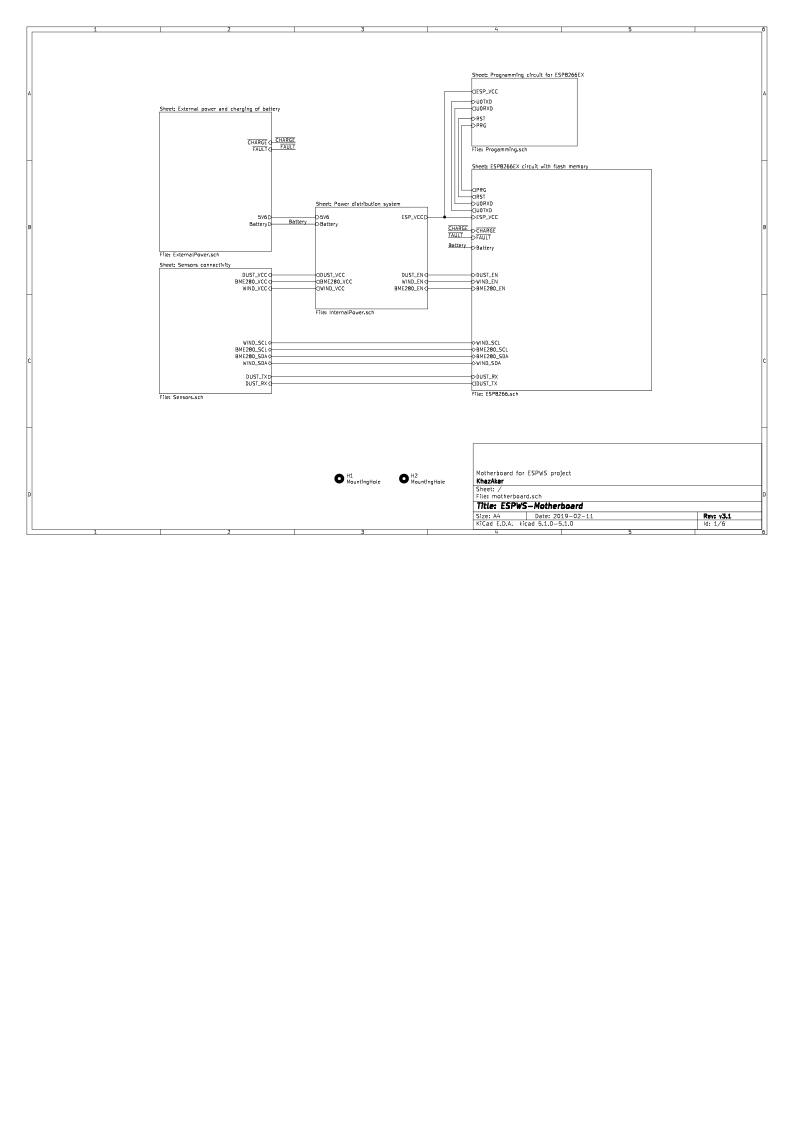
\includegraphics[scale=0.4]{img/first.png}
\end{center}
\end{frame}
\begin{frame}
	\frametitle{PCB}
	Zaprojektowano płytkę drukowaną z wykorzystaniem 4 warstw, w następującej konfiguracji: Sygnał - Masa - Zasilanie - Sygnał
	\begin{center}
		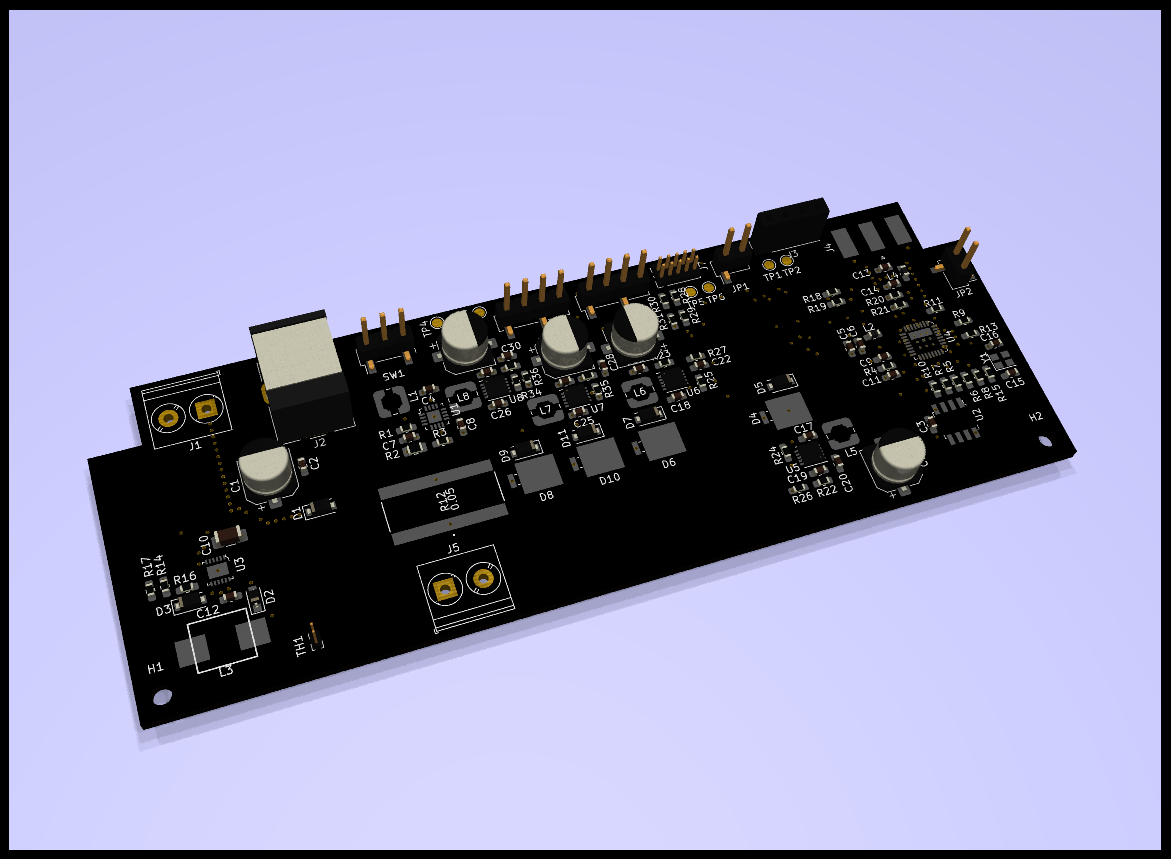
\includegraphics[scale=0.15]{img/render.png}
	\end{center}
\end{frame}
\begin{frame}
\frametitle{Kod źródłowy}
	Kod źródłowy projektu został napisany z wykorzystaniem Eclipse IDE i pluginu Sloeber. Wykorzystano biblioteki Arduino z uwagi na prostotę implementacji i duże możliwości dostępnych, dodatkowych bibliotek.
		\begin{center}
		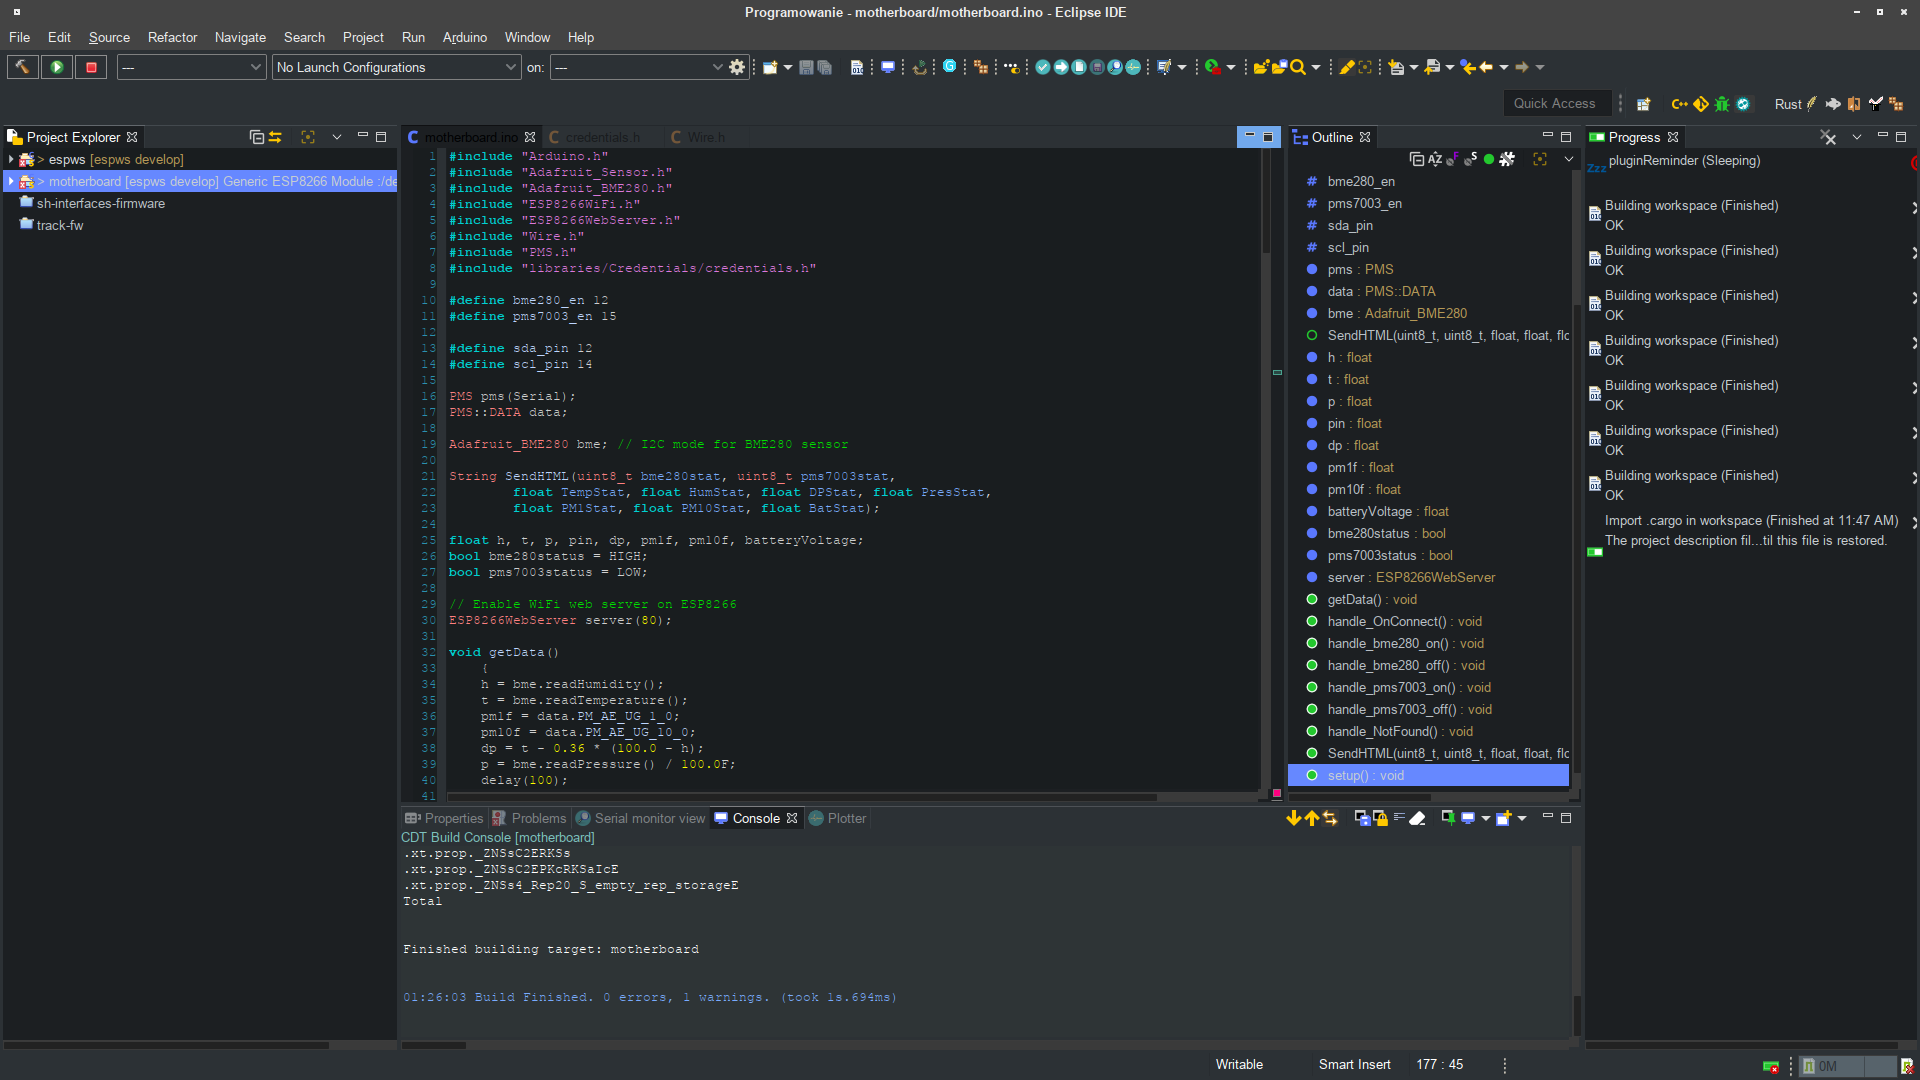
\includegraphics[scale=0.1]{img/eclipse.png}
	\end{center}
\end{frame}
\begin{frame}
	\frametitle{Działanie projektu}
	Menu całości jest proste i przejrzyste - pozwala na podgląd pomiarów oraz parametrów, jak i na kontrolę pinów kontrolujących przetwornice DC-DC. Dostępny jest podgląd temperatury, ciśnienia, wilgotności, zanieczyszczeń PM1 oraz PM10. Z parametrów dostępny jest pomiar napięcia na baterii. Umożliono także kontrolę nad zasilaniem czujników.
			\begin{center}
		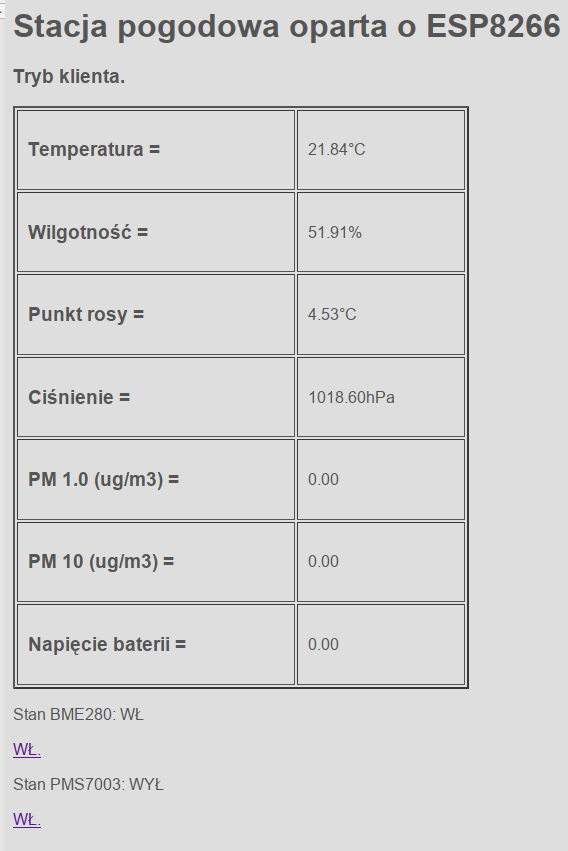
\includegraphics[scale=0.15]{img/app01.png}
	\end{center}
\end{frame}
\begin{frame}
\frametitle{Napotkane problemy}
	Wystąpiło kilka problemów:
	\begin{itemize}
		\item Do zaprogramowania układu potrzeba przylutować kilka dodatkowych przewodów; wyprowadzone pierwotnie piny są niewystarczające
		\item Sygnały \text{$\sim$CHARGE} i \text{$\sim$FAULT} nie mogą być wykorzystane - brak rezystorów podciągających
		\item Liczne przelotki na ścieżce wejściowej z panelu słonecznego - dodają niepotrzebną rezystancję w tej konfiguracji
	\end{itemize}
\end{frame}
\begin{frame}
\frametitle{Możliwe rozwiązania problemów}
	Każdy z tych problemów da się rozwiązać jedynie przez modyfikację schematu i płytki drukowanej, a mianowicie:
	\begin{itemize}
		\item Wyprowadzenie wszystkich niezbędnych sygnałów programowania;
		\item Dodanie rezystorów podciągających do sygnałów \text{$\sim$CHARGE} i \text{$\sim$FAULT};
		\item Usunięcie przelotek z ścieżki i poszerzenie jej tak, żeby mogła spełniać założenia.
	\end{itemize}
\end{frame}
\begin{frame}
\frametitle{Przyszłość projektu}
	Projekt będzie cały czas rozwijany w wolnym czasie. Będą tworzone nowe rewizje schematu oraz płytek drukowanych dla lepszego przystosowania projektu do sprzedaży gotowych produktów z jego wykorzystaniem.
\end{frame}
\end{document}